\section{Background}
\label{background}

The power grid is composed of power generation, transmission, distribution and loads. Traditionally, power is generated in mass quantities from hydro, coal, nuclear, and gas sources. The power is then transmitted at high voltages to distribution systems where the power is distributed to residential and commercial consumers. As the power grid is moving towards a smarter grid, the efficient energy management is increasingly dependent on the underlying communication network supporting reliable information transfer among the various entities in the grid.

With distributed power generation---such as solar and wind energy---and more storage technology, there is a need for understanding the state of the power network in real time. A challenge with the integration of such generation, is the uncertainty and intermittency of the availability of power generation.
In order to combat this challenge, there needs to be an infrastructure that allows for the monitoring and control of the system state. To do this effectively, requires a reliable and resilient communication network.

Researchers have developed systems to co-simulate the power and network components of the smart grid \cite{DSSco-sim, DSS-RT-HIL, RT-SmartGrid, GECO, EPOCHS, FNCS, FNCS-algos}. \cite{Mets2014} surveys the existing technologies and motivations for co-simulation.

In \cite{DSS-RT-HIL}, a system is proposed using OpenDSS to allow for sending real-time signals to hardware integrating with simulation.
Real time simulators are used for hardware-in-the-loop simulations, allowing for simulation-emulation closer to the real system \cite{RT-SmartGrid}. This gives high fidelity, but requires power equipment and often specific simulator hardware.
While real-time simulators exist, they are costly and often require specific hardware to operate, our challenge is to design a hardware-in-the-loop testbed that can use standard electric power simulators that run slower than real-time while maintaining temporal fidelity.

In \cite{GECO}, the authors create a co-simulation between PSLF and ns-2.
They use a global event driven mechanism for sending synchronization messages between the two simulators.
In simulation, events are sorted by time stamps, typically in a priority queue and are executed as fast as possible without regard to the wall clock.

EPOCHS \cite{EPOCHS} uses commercial power simulators to co-simulate network and power systems through the use of agents.
%While agents are not new to simulation,
This platform uses agents to effectively co-simulate power and communication elements.
The authors define agents as having the properties of autonomy and interaction.
That they exhibit properties of mobility, intelligence, adaptivity and communication.
In our design, our models run real processes on real hardware but can influence and extract values from the power simulator.
This allows for us to make use of agents to as entities that exist in both systems.

FNCS \cite{FNCS} is a federated approach for co-simulation of power and electrical simulators by combining multiple power simulators, both distribution and transmission and use ns-3 as a communication simulator.
In \cite{FNCS-algos}, the same authors improve the synchronization between systems.
The difference is that our approach is focused on running real network processes which has different synchronization challenges due to the inherent difference between the execution mechanisms in simulation and real-time processes.

There are two main features that set our design apart from the existing tools.
The first is that we are using real hardware for networking components rather than a simulator.
The second is that our testbed's design works without real-time simulators making our apporach general and low-cost.



\if 0
\section{motivation}
\label{motivation}
\fi


\section{Project Goals}

While simulation systems offer a convinient and low cost method of perfoming evaluation on models of systems it lacks the fidelity that real systems contain.

This project aims to achieve the following:
\begin{itemize}  
  \item create a distributed system composed of embedded linux devices including general purpose and router devices.
  \item provide synchronization solution for real-time processes to synchronize with a descrete time step solution electric power simulator.
\end{itemize}


The challenges in the creation of such testbed stem for the synchronization issues between nodes in the distributed system, the processes running on the nodes, and the simulator. Specifically we will implement the following in a testbed consisting of 5 nodes, a embedded router, 2 Banana Pi devices, and 2 Raspberry Pi linux devices:

\begin{itemize}
\item Creating a kernel module that provides a user-space utility for sending hardware interrupts between the devices in the system.
The distributed synchronization between the devices is decentralized with the kernel module. 
  \item Time synchronization strategy with the simulation server.
  \item Modify the scheduler to control process execution.
\end{itemize}

\begin{figure*}
  \centering
  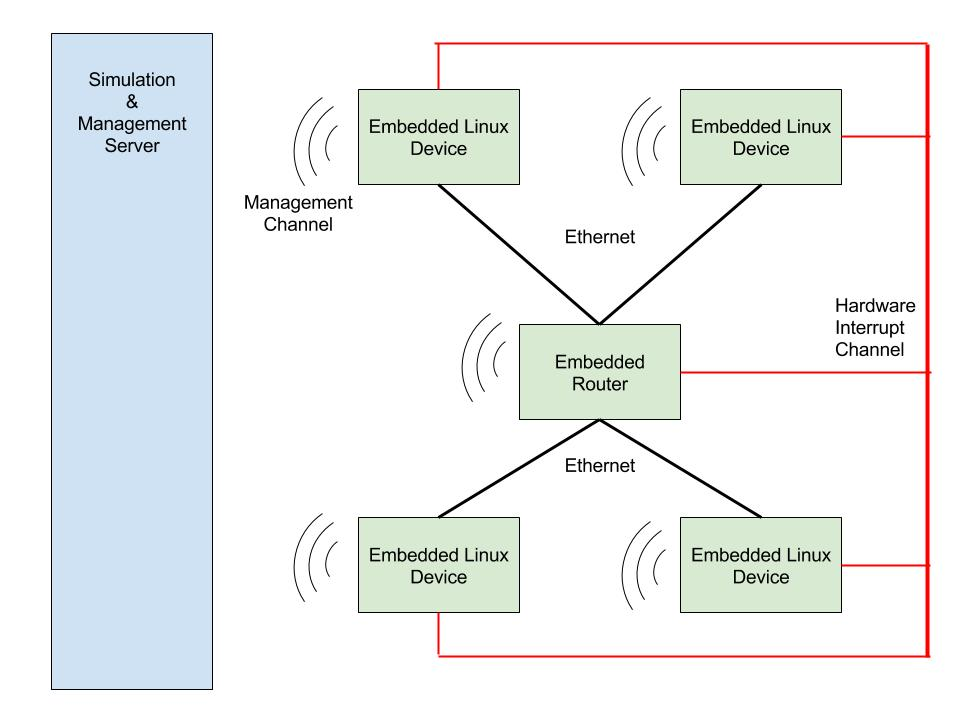
\includegraphics[scale=0.5]{architecture.jpg}
  \caption{
    Architecture of distributed system composed of 3 communication channels: Ethernet, wireless management, and direct hardware connection
    }
\end{figure*}


\section{Project Execution Plan}

For this project we have the following rough project plan:

\begin{itemize}
\item February:
\begin{itemize}
  \item implement kernel module
  \item collect information regarding clock skewness
\end{itemize}

\item March:
\begin{itemize}
  \item create time synchronization strategy
  \item modify scheduler
\end{itemize}

\item April:
\begin{itemize}
  \item perform system evaluation
  \item create use case
  \item presentation preparation
\end{itemize}

\end{itemize}


